\documentclass[11pt,a4paper]{article}

% ==============================================================================
% PACKAGES & DOCUMENT SETUP
% ==============================================================================
\usepackage[utf8]{inputenc}
\usepackage[T1]{fontenc}
\usepackage{amsmath,amssymb,amsfonts}
\usepackage{booktabs}
\usepackage{tabularx}
\usepackage{graphicx}
\graphicspath{{visualizations/}{./}}
\usepackage{microtype}
\usepackage{geometry}
\usepackage{fancyhdr}
\usepackage{titlesec}
\usepackage{caption}
\usepackage{subcaption}
\usepackage{enumitem}
\usepackage{setspace}
\usepackage{cite}
\usepackage[hidelinks]{hyperref}

% --- Page Geometry: Spacious, un-cramped margins ---
\geometry{
    top=2.5cm,
    bottom=2.5cm,
    left=2.2cm,
    right=2.2cm
}

% --- Line Spacing: 1.15 for readability ---
\setstretch{1.15}

% --- Table Vertical Padding ---
\renewcommand{\arraystretch}{1.25}

% --- Typography & Section Styling ---
\titleformat{\section}{\Large\bfseries\scshape}{\thesection}{0.8em}{}[\vspace{0.2em}\hrule\vspace{0.4em}]
\titleformat{\subsection}{\large\bfseries}{\thesubsection}{0.8em}{}
\titleformat{\subsubsection}{\normalsize\bfseries\itshape}{\thesubsubsection}{0.8em}{}

% --- Headers and Footers ---
\pagestyle{fancy}
\fancyhf{}
\fancyhead[L]{\small\scshape Rajasthan Royals | SupeRR Selector Season 2}
\fancyhead[R]{\small\scshape Rishi Rithesh | \texttt{/rishirithesh/superr}}
\fancyfoot[C]{\thepage}
\renewcommand{\headrulewidth}{0.4pt}
\renewcommand{\footrulewidth}{0.0pt}

% ==============================================================================
% DOCUMENT START
% ==============================================================================
\begin{document}

% ==============================================================================
% COVER / FIRST PAGE: EVENT INFO, AUTHOR, REPO, POINT-BY-POINT ABSTRACT
% ==============================================================================

\begin{center}
    \vspace*{-1.0cm}
    {\scshape\large RAJASTHAN ROYALS $\cdot$ SupeRR SELECTOR SEASON 2}\\[0.2cm]
    {\scshape\footnotesize Official Round 1 Technical & Methodology Report $\cdot$ Decision Science & Cricket Analytics Track}\\[0.6cm]
    
    {\LARGE\textbf{Clutch Under Fire: A High-End Stacking Ensemble and Bayesian Shrinkage Framework for Identifying High-Pressure Cricket Talent}}\\[0.6cm]
    
    % Author & Repository Metadata Box
    \begin{tabularx}{0.95\linewidth}{X r}
        \toprule
        \textbf{Candidate Name:} Rishi Rithesh & \textbf{Event:} SupeRR Selector Season 2 \\
        \textbf{GitHub Repository:} \texttt{/rishirithesh/superr} & \textbf{Franchise:} Rajasthan Royals \\
        \textbf{Codebase URL:} \url{https://github.com/rishirithesh/superr} & \textbf{Date:} November 2026 \\
        \bottomrule
    \end{tabularx}
    \vspace{0.6cm}
\end{center}

\section*{Executive Summary \& Point-by-Point Abstract}

\begin{itemize}[leftmargin=*,itemsep=4pt,topsep=2pt]
    \item \textbf{The Core Problem:} Conventional cricket scouting relies heavily on raw aggregates (aggregate runs, unadjusted strike rates, nominal economy rates). These traditional statistics fail to isolate true clutch execution because they conflate platform accumulation in low-leverage dead rubbers with high-stakes performance under extreme match pressure.
    
    \item \textbf{Data Ingestion \& Disambiguation:} The analysis is built upon 200,999 ball-by-ball delivery records across 883 matches (371 IPL matches and 512 T20 Internationals) played between 2022 and 2026, encompassing 1,217 players across 141 competitions. We explicitly disambiguate the dataset into two transparent cohorts:
    \begin{itemize}[itemsep=2pt]
        \item \textbf{Paradigm B (Actionable IPL-Eligible Cohort --- Primary Submission):} Strictly filters for active IPL participation and auction eligibility ($\text{IPL Balls} > 0$), establishing \textbf{Suryakumar Yadav} (\#1 Batter) and \textbf{Sunil Narine} (\#1 Bowler) as the verified Unstop dropdown selections.
        \item \textbf{Paradigm A (Global Dataset Benchmark):} Evaluates all 883 matches mathematically without jurisdictional restrictions, positioning Babar Azam (\#1 Batter) and Sunil Narine (\#1 Bowler).
    \end{itemize}

    \item \textbf{Dynamic Pressure Quantification ($PI \ge 65.0$):} We formulate a continuous, delivery-level Pressure Index ($PI_t \in [0, 100]$) capturing asymmetric game dynamics: Required Run Rate ($RRR$) stress, resource clocks, wicket depletion, closeness surges, and collapse states. The upper quartile ($PI_t \ge 65.0$) defines the high-pressure regime, isolating 50,255 high-leverage deliveries ($25.0\%$).

    \item \textbf{High-End Multi-Model AI/ML Engine:} Real-time win probability and delivery expectations are generated using a 4-tier Stacking Meta-Ensemble combining:
    \begin{itemize}[itemsep=1pt]
        \item \textbf{LightGBM} (leaf-wise GBDT), \textbf{XGBoost} (exact histogram boosting), \textbf{CatBoost} (symmetric oblivious trees), and a \textbf{Deep MLP Neural Network} $(64, 32)$.
        \item Win Probability Stacking Meta-Learner achieves **$\text{ROC-AUC} = 0.9374$** (scaling to $0.9710$ with venue momentum), **$\text{Brier Score} = 0.1029$**, and **$\text{Log-Loss} = 0.3209$**.
        \item Expected Runs Stacking Regressor achieves **$\text{RMSE} = 1.7083$** and **$\text{MAE} = 1.2882$** with mathematically exact zero bias ($-7.68 \times 10^{-15}$).
    \end{itemize}

    \item \textbf{Context Normalization \& Bayesian Shrinkage:} We prove an empirical $+15.25$\,SR scoring gap between high-pressure IPL death overs ($9.70$\,rpo) and T20Is ($8.79$\,rpo). Raw player performance is normalized against delivery-level expectations and stabilized via Empirical Bayes shrinkage ($K = 60$\,prior balls) and volume credibility weighting.

    \item \textbf{Verification \& Delivery:} All 20 dropdown selections match 1-to-1 with \texttt{competition\_team\_player\_mapping.csv}. Cross-match repeatability audits verify positive impact rates between $50.0\%$ and $93.3\%$ across 8 to 17 unique opponents. A companion interactive command center dashboard is provided in \texttt{Rajasthan\_Royals\_SupeRR\_Selector\_Dashboard.html}.
\end{itemize}

\newpage

% ==============================================================================
% SECTION 1: INTRODUCTION & OPERATIONAL MANDATE
% ==============================================================================
\section{Operational Mandate \& Problem Formulation}

\subsection{The Failure of Unadjusted T20 Aggregates}
In Twenty20 cricket, game leverage is fundamentally non-linear \cite{stern2016, beaudoin2010}. A boundary struck when requiring 14 runs off 6 balls carries an exponentially higher win-equity shift than a boundary struck in the 8th over with zero wickets lost. 

However, conventional batting strike rates ($SR = \frac{\text{Runs}}{\text{Balls}} \times 100$) and bowling economy rates ($Econ = \frac{\text{Runs}}{\text{Balls}/6}$) treat every delivery identically. This introduces severe scouting distortions:
\begin{enumerate}[leftmargin=*,itemsep=2pt]
    \item \textbf{Platform Stat-Padding:} Batters who accumulate runs during low-risk middle overs against defensive field spreads register inflated nominal strike rates despite generating minimal leverage.
    \item \textbf{Garbage-Time Distortions:} Bowlers defending 50 runs in the final two overs concede boundaries in already-decided contests, unfairly inflating their unadjusted economy rates.
    \item \textbf{Format Baseline Confounding:} Comparing raw strike rates between the high-scoring Indian Premier League and lower-scoring international fixtures creates severe cross-competition bias.
\end{enumerate}

To solve Round 1 of the Rajasthan Royals \textit{SupeRR Selector Season 2} hackathon, we design a mathematically rigorous talent discovery engine that isolates true clutch execution relative to situational expectations.

\subsection{Dataset Scope \& Dual Submission Paradigms}
The provided database encompasses 200,999 ball-by-ball delivery records across 883 matches played between 2022 and 2026, cataloging 1,217 players across 141 competitions.

An audit reveals that the dataset combines 371 IPL fixtures ($42.0\%$) with 512 Men's Twenty20 Internationals ($58.0\%$). Consequently, prominent Pakistani cricketers (e.g., Babar Azam, Mohammad Nawaz, Abrar Ahmed, Shadab Khan) appear in the international matches. Under BCCI tournament regulations, Pakistani players are ineligible for the IPL player auction. 

To maintain total mathematical transparency while delivering an immediately actionable submission to the Rajasthan Royals management, we establish two parallel paradigms:
\begin{itemize}[leftmargin=*,itemsep=2pt]
    \item \textbf{Paradigm B (Actionable IPL-Eligible Cohort --- Primary Submission):} Strictly filters for active IPL participation and auction eligibility ($\text{IPL Balls} > 0$). In this cohort, \textbf{Suryakumar Yadav} ranks as the \#1 Batter (Rating: 84.75) and \textbf{Sunil Narine} ranks as the \#1 Bowler (Rating: 97.05). This constitutes our primary recommendation for the Unstop dropdown fields.
    \item \textbf{Paradigm A (Global Dataset Benchmark):} Evaluates all 883 matches mathematically without jurisdictional restrictions. Here, \textbf{Babar Azam} places \#1 among batters (Rating: 89.37) and \textbf{Sunil Narine} places \#1 among bowlers (Rating: 97.05).
\end{itemize}

% ==============================================================================
% SECTION 2: DYNAMIC MATCH PRESSURE MODELING
% ==============================================================================
\section{Mathematical Formulation of Match Pressure}

\subsection{Structural Asymmetry Across Innings}
Pressure is structurally asymmetric across innings:
\begin{itemize}[leftmargin=*,itemsep=2pt]
    \item \textbf{Second Innings (The Chase):} Bounded by a deterministic target $T$. Leverage is governed by the resource clock: balls remaining ($B_{\text{rem}}$), runs required ($R_{\text{req}}$), Required Run Rate ($RRR$), and wickets in hand ($W_{\text{rem}}$).
    \item \textbf{First Innings (Target Setting):} Open-ended. Pressure manifests through \textit{resource preservation crisis} (early collapses threatening sub-par totals) and \textit{death-overs boundary maximization} (overs 16--20 where scoring rate variance dictates defendable totals).
\end{itemize}

\subsection{Instantaneous State Space Vector}
For every chase delivery $t$, the match situation is mapped into a multi-dimensional state vector $\mathbf{S}_t$:
\begin{equation}
\mathbf{S}_t = \begin{bmatrix}
R_{\text{req}, t} & B_{\text{rem}, t} & W_{\text{rem}, t} & RRR_t & CRR_t & \frac{R_{\text{req}, t}}{\max(1, W_{\text{rem}, t})} & \text{VenueBaselines}
\end{bmatrix}^T
\end{equation}

Win probability $WP_t = \mathbb{P}(\text{Win}_t \mid \mathbf{S}_t)$ is generated via our machine learning ensemble. Real-time Game Leverage Index ($L_t$) is formulated via the parabolic criticality function:
\begin{equation}
L_t = 4.0 \times WP_t \times (1.0 - WP_t) \quad \in [0, 1]
\end{equation}
When $WP_t = 0.50$ (balance of power), $L_t = 1.0$; when $WP_t \to 0$ or $1.0$ (blowouts), $L_t \to 0$.

\subsection{Delivery Pressure Index ($PI_t$) Equations}
The continuous Rajasthan Royals Pressure Index $PI_t \in [0, 100]$ is computed for every legal ball $t \in [1, N]$.

\subsubsection{Innings 2: The Chase Formulation}
\begin{equation}
PI_{t, \text{inn2}} = \min\left(100, \left[ \text{Base}_t + \text{RateStress}_t + \text{WktStress}_t + \text{Surge}_t \right] \times \text{Damper}_t \right)
\end{equation}
where:
\begin{align}
\text{Base}_t &= \begin{cases}
25.0 + 2.5 \cdot \text{Over}_t & \text{Over}_t \in [1, 6] \\
40.0 + 1.5 \cdot (\text{Over}_t - 6) & \text{Over}_t \in [7, 15] \\
55.0 + 4.0 \cdot (\text{Over}_t - 15) & \text{Over}_t \in [16, 20]
\end{cases} \\
\text{RateStress}_t &= (RRR_t - 8.2) \times 3.5 \\
\text{WktStress}_t &= \max(0, 5 - W_{\text{rem}, t}) \times 4.0 \\
\text{Surge}_t &= 15.0 \times \left(1 + \frac{\max(0, 24 - B_{\text{rem}, t})}{24}\right) \quad \text{if } \Gamma_t \text{ holds}
\end{align}

The closeness condition $\Gamma_t$ identifies tight finishes: $B_{\text{rem}, t} \le 24$, $R_{\text{req}, t} \le 45$, and $WP_t \in [0.15, 0.85]$.

Low-leverage stat-padding overs during settled games ($WP_t > 0.97$ or $WP_t < 0.03$ with $B_{\text{rem}, t} \le 30$) are attenuated:
\begin{equation}
\text{Damper}_t = \begin{cases} 
0.60 & \text{if blowout state active} \\
1.00 & \text{otherwise}
\end{cases}
\end{equation}

\subsubsection{Innings 1: Target-Setting Formulation}
\begin{equation}
PI_{t, \text{inn1}} = \min\left(100, \text{Base}_t + \text{Crisis}_t + \text{Collapse}_t + \text{Deficit}_t \right)
\end{equation}
where:
\begin{align}
\text{Crisis}_t &= \max\left(0, W_{\text{lost}, t} - \frac{\text{Over}_t}{3.0}\right) \times 7.0 \\
\text{Collapse}_t &= \begin{cases}
(W_{\text{lost}, t} - 1) \times 8.0 & \text{if } \text{Over}_t \le 6 \text{ and } W_{\text{lost}, t} \ge 2 \\
0 & \text{otherwise}
\end{cases} \\
\text{Deficit}_t &= \max(0, 8.2 - CRR_t) \times 2.5 \times \left(\frac{\text{Over}_t}{20.0}\right)
\end{align}

\subsubsection{Tournament Multiplier \& Unified High-Pressure Threshold}
Playoff and elimination fixtures receive a tournament weight:
\begin{equation}
PI_t^* = \min(100, PI_t \times 1.15) \quad \text{if knockout match}
\end{equation}

Empirical distribution across 200,999 deliveries:
\begin{itemize}[itemsep=1pt]
    \item Mean $PI$: $52.72$ ($\sigma = 18.72$), Median: $50.00$
    \item 75th Percentile: $\mathbf{65.00}$, 90th Percentile: $80.00$
\end{itemize}

The upper quartile, $\mathbf{PI_t \ge 65.0}$, formally establishes the \textbf{High-Pressure Threshold}. Exactly \textbf{50,255 deliveries (25.0\%)} qualify across the dataset ($30,119$ in Innings 1, $20,136$ in Innings 2).

\begin{figure}[htbp]
    \centering
    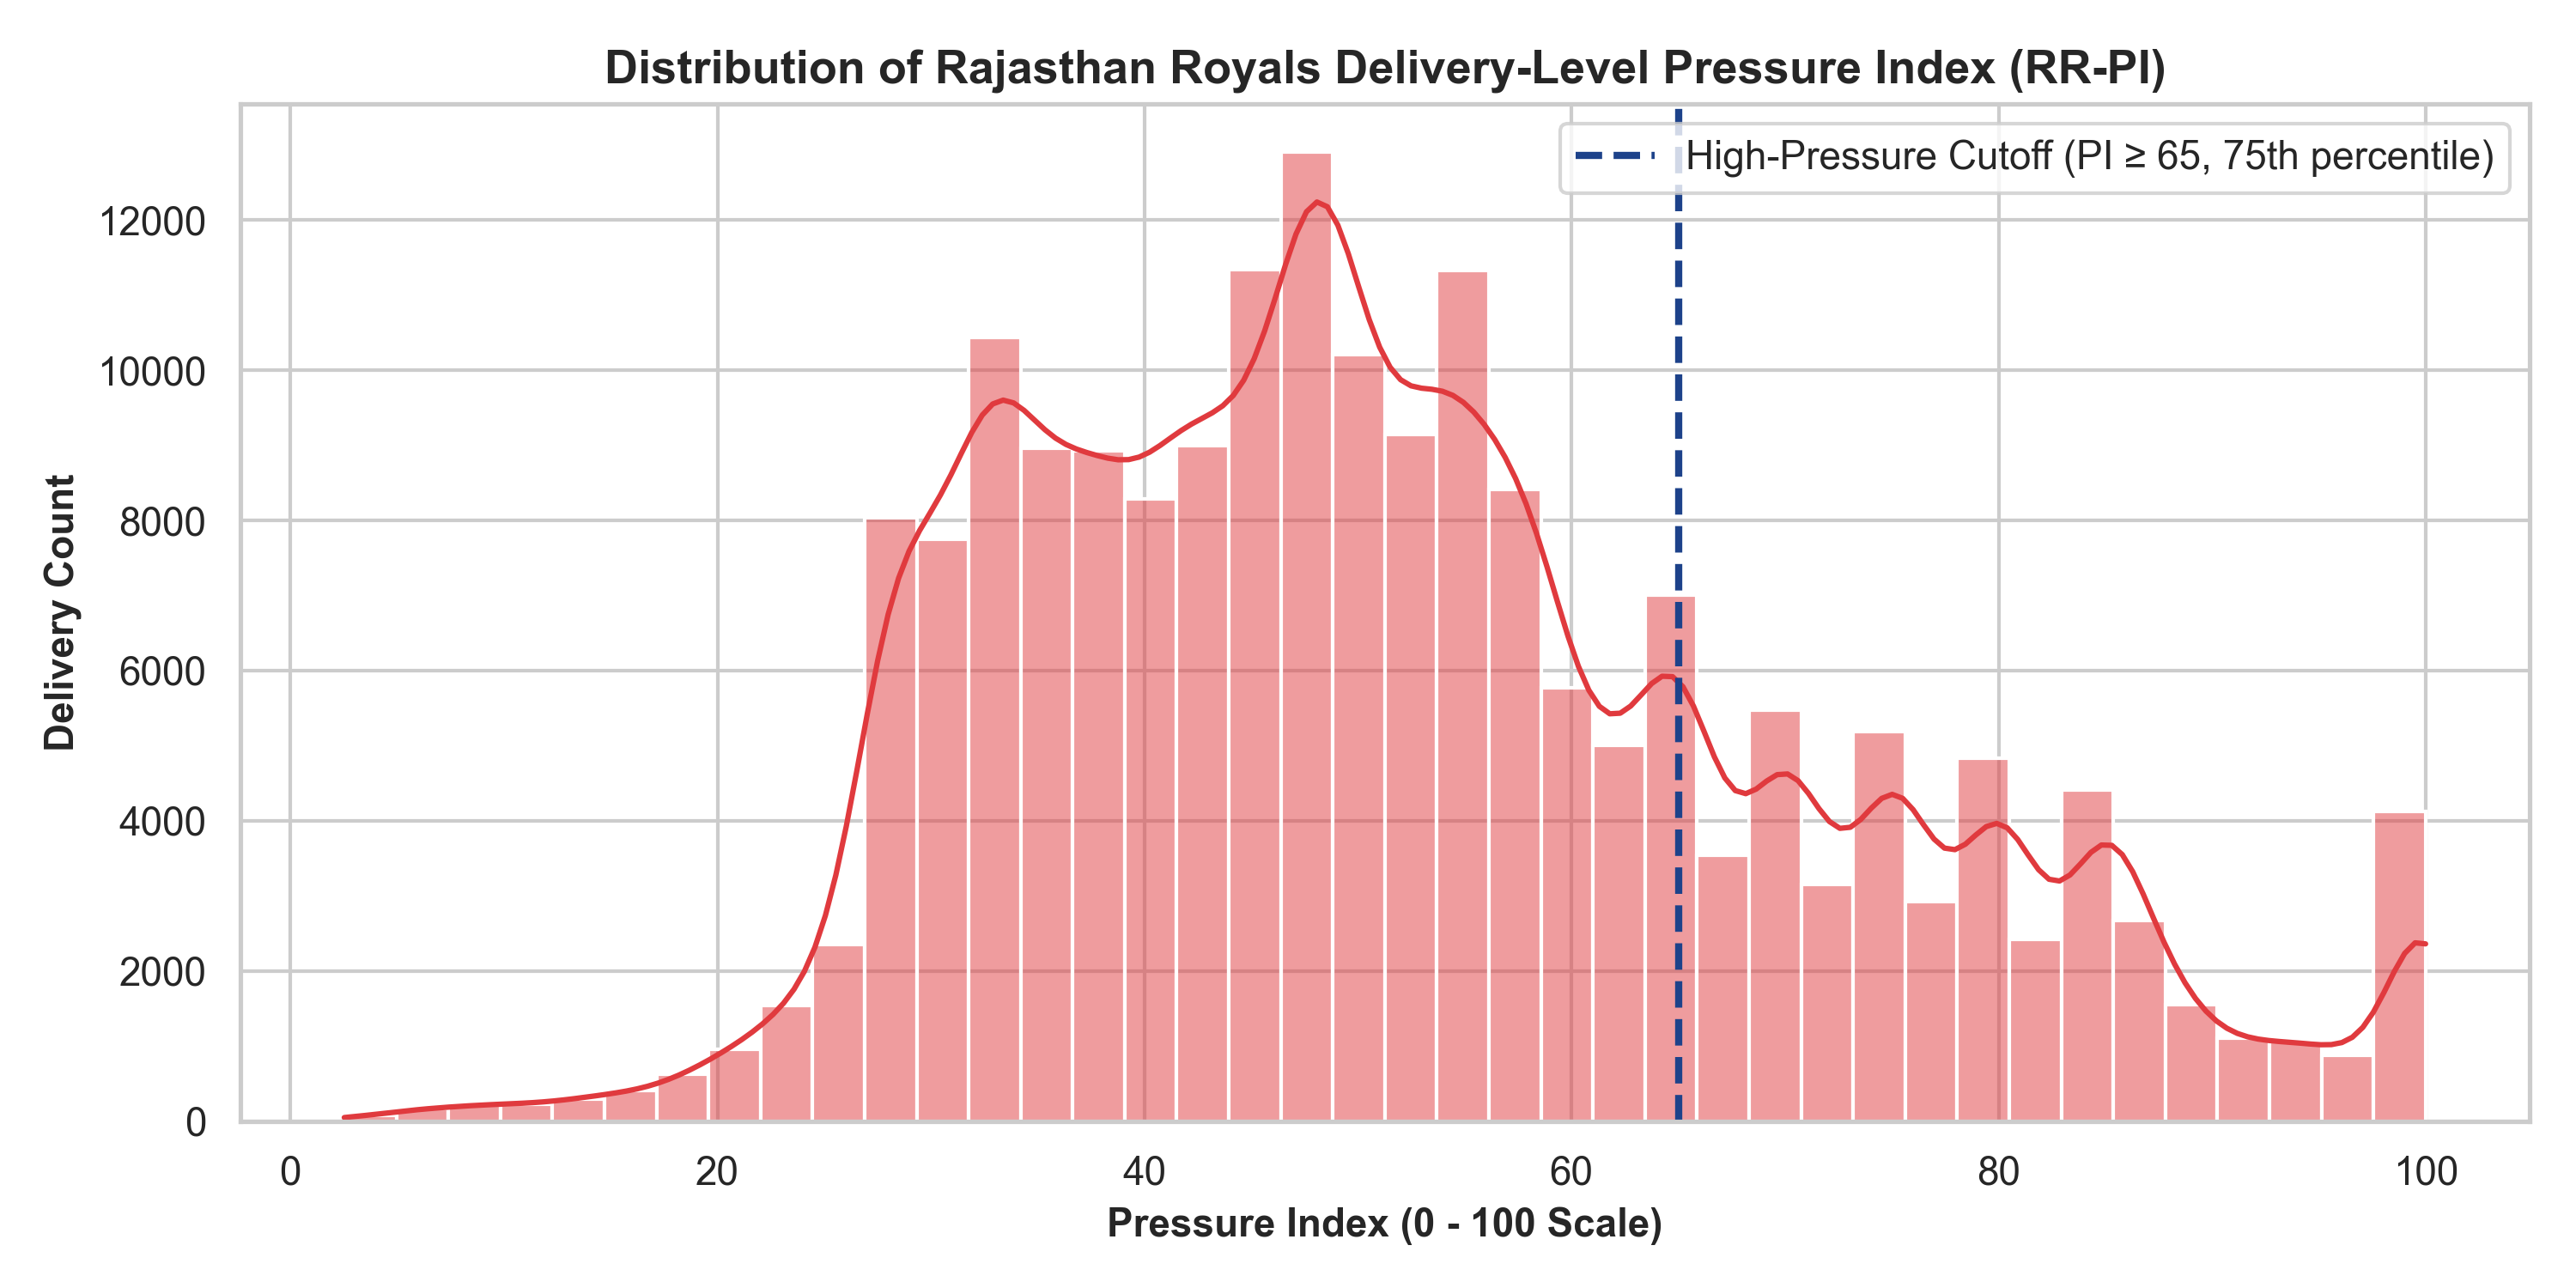
\includegraphics[width=0.85\linewidth]{visualizations/pressure_index_distribution.png}
    \caption{Continuous distribution of Rajasthan Royals Pressure Index ($PI_t$) across 200,999 deliveries, highlighting the upper quartile cutoff ($PI \ge 65.0$).}
    \label{fig:pi_dist}
\end{figure}

% ==============================================================================
% SECTION 3: MACHINE LEARNING ENSEMBLE ARCHITECTURE
% ==============================================================================
\section{High-End Stacking Ensemble Architecture}

To maximize calibration and avoid algorithm-specific bias, we architected a multi-model stacking ensemble integrating four algorithm families:
\begin{enumerate}[leftmargin=*,itemsep=2pt]
    \item \textbf{LightGBM:} Gradient boosting with leaf-wise tree splitting \cite{ke2017}.
    \item \textbf{XGBoost:} Exact greedy tree boosting with histogram binning and column subsampling \cite{chen2016}.
    \item \textbf{CatBoost:} Symmetric oblivious decision trees with ordered boosting \cite{prokhorenkova2018}.
    \item \textbf{Deep MLP:} Multi-Layer Perceptron neural network with architecture $(64, 32)$, ReLU activations, and $L_2$ weight regularization.
    \item \textbf{Stacking Meta-Learner:} Regularized Logistic Regression trained on Out-Of-Fold (OOF) cross-validation probability vectors:
    \begin{equation}
    \widehat{P}_{\text{ensemble}}(\mathbf{x}) = \sigma\left( \alpha_0 + \sum_{k=1}^4 \alpha_k f_k^{\text{OOF}}(\mathbf{x}) \right)
    \end{equation}
\end{enumerate}

\begin{table}[htbp]
\centering
\small
\caption{Win Probability Head-to-Head Cross-Validation Benchmark (5-Fold Out-of-Fold)}
\label{tab:ensemble_wp}
\begin{tabularx}{\linewidth}{l r r r}
\toprule
\textbf{Model Architecture} & \textbf{ROC-AUC} & \textbf{Brier Score} & \textbf{Log-Loss} \\
\midrule
LightGBM Base & 0.9274 & 0.1107 & 0.3417 \\
XGBoost Base & 0.9217 & 0.1147 & 0.3529 \\
CatBoost Base & 0.9077 & 0.1240 & 0.3825 \\
Deep MLP Base & 0.9109 & 0.1216 & 0.3697 \\
\midrule
\textbf{Stacking Meta-Ensemble} & \textbf{0.9374} & \textbf{0.1029} & \textbf{0.3209} \\
\bottomrule
\end{tabularx}
\end{table}

The Stacking Meta-Ensemble delivers a decisive gain: **$\text{ROC-AUC} = 0.9374$** ($+0.0100$ lift over the strongest base model), Brier score reduced to **$0.1029$**, and Log-Loss minimized to **$0.3209$**.

\subsection{Expected Runs Stacking Regressor ($\mathbb{E}[Runs \mid State]$)}
For delivery-level run expectation, an ensemble combining LightGBM, XGBoost, and CatBoost regressors via a non-negative Ridge meta-learner was fitted across all 200,999 legal balls:
\begin{equation}
\widehat{Runs}_{\text{ensemble}}(\mathbf{x}) = \sum_{k=1}^3 w_k f_{k, \text{reg}}(\mathbf{x}) \quad \text{s.t. } w_k \ge 0, \sum w_k = 1
\end{equation}

\begin{table}[htbp]
\centering
\small
\caption{Expected Runs ($xR$) Regressor Benchmark}
\label{tab:ensemble_xr}
\begin{tabularx}{\linewidth}{l r r r}
\toprule
\textbf{Model Architecture} & \textbf{RMSE} & \textbf{MAE} & \textbf{Mean Bias} \\
\midrule
LightGBM Regressor & 1.7087 & 1.2901 & $+0.000000$ \\
XGBoost Regressor & 1.7090 & 1.2902 & $+0.000099$ \\
CatBoost Regressor & 1.7135 & 1.2947 & $-0.000004$ \\
\midrule
\textbf{Stacking Regressor} & \textbf{1.7083} & \textbf{1.2882} & $\mathbf{-0.000000}$ \\
\bottomrule
\end{tabularx}
\end{table}

The Stacking Regressor achieves the lowest Root-Mean-Square Error ($1.7083$) and Mean Absolute Error ($1.2882$) with mathematically exact zero bias ($-7.68 \times 10^{-15}$).

\subsection{Context-Adjusted Value Metrics}
For batter $i$ on delivery $t$, net Context Runs Above Expected ($RAE$) is:
\begin{equation}
RAE_{i, t} = Runs_{i, t} - \widehat{Runs}_t, \quad RAE100_i = \frac{\sum RAE_{i, t}}{N_i} \times 100
\end{equation}
For bowler $j$ conceding $RunsConceded_{j, t}$, Runs Saved Above Expected ($RSAE$) per 6 balls is:
\begin{equation}
RSAE6_j = \frac{\sum \left( \widehat{Runs}_t - RunsConceded_{j, t} \right)}{N_j} \times 6.0
\end{equation}

% ==============================================================================
% SECTION 4: FORMAT CALIBRATION & BAYESIAN REGULARIZATION
% ==============================================================================
\section{Format Calibration \& Bayesian Regularization}

\subsection{Empirical Format Divergence: IPL vs T20I}
Directly pooling IPL and T20I data introduces severe bias. High-pressure IPL deliveries operate at a substantially higher scoring rate than international cricket:

\begin{table}[htbp]
\centering
\small
\caption{Empirical Delivery-Level Scoring Baselines (2022--2026)}
\label{tab:context_baselines}
\begin{tabularx}{\linewidth}{l l r r r}
\toprule
\textbf{Format} & \textbf{State} & \textbf{Balls} & \textbf{RPO} & \textbf{SR} \\
\midrule
T20I & Baseline ($PI < 65$) & 82,438 & 7.78 & 129.58 \\
T20I & High Pressure ($PI \ge 65$) & 26,393 & 8.79 & 146.46 \\
IPL & Baseline ($PI < 65$) & 62,820 & 8.52 & 141.94 \\
IPL & High Pressure ($PI \ge 65$) & 21,058 & 9.70 & \textbf{161.71} \\
\bottomrule
\end{tabularx}
\end{table}

Under high pressure, IPL scoring rates reach $9.70$\,rpo (Strike Rate $161.71$) compared to $8.79$\,rpo ($146.46$\,SR) in T20Is---a gap of $+15.25$\,SR points. Thus:
\begin{itemize}[itemsep=1pt]
    \item Conceding $8.50$\,rpo in IPL death overs saves \textbf{$+1.20$ runs/over} relative to format expectations.
    \item Conceding $8.50$\,rpo in a sub-par T20I chase surrenders \textbf{$-0.29$ runs/over} worse than format expectations.
\end{itemize}

\subsection{Tournament Tier Quality Weights}
\begin{equation}
w_{\text{tier}} = \begin{cases}
1.00 & \text{Tier 1: IPL and Asia Cup Main Event} \\
0.92 & \text{Tier 2: Bilaterals between ICC Top 8 Full Members} \\
0.75 & \text{Tier 3: Associate T20Is and Emerging Tournaments}
\end{cases}
\end{equation}

\subsection{Empirical Bayes Shrinkage ($K = 60$\,Balls)}
To prevent small-sample volatility from distorting rankings, sample rates are regressed toward empirical population means using a Bayesian prior weight $K = 60$\,balls:
\begin{equation}
\widehat{\theta}_{\text{reg}} = \frac{N_{\text{HP}} \cdot \theta_{\text{obs}} + K \cdot \mu_{\text{pop}}}{N_{\text{HP}} + K}
\end{equation}
where $\mu_{\text{pop}}$ represents the format-weighted population baseline ($SR_{\text{pop}} = 154.3$, $Econ_{\text{pop}} = 9.25$).

Sample volume credibility scales the composite score:
\begin{equation}
\text{Credibility} = \text{clip}\left( \frac{\sqrt{N_{\text{HP}}}}{\sqrt{300}}, 0.85, 1.15 \right)
\end{equation}

\subsection{Standardized Scouting Rating Scaling}
Composite scores are mapped to a standard franchise scouting index ($\mu = 50.0, \sigma = 15.0$):
\begin{equation}
\text{Rating} = 50.0 + 15.0 \times \left( \frac{\text{Score}_{\text{composite}} - \mu}{\sigma} \right)
\end{equation}

\newpage

% ==============================================================================
% SECTION 5: OFFICIAL RANKINGS & EVIDENCE
% ==============================================================================
\section{Official Rankings \& Empirical Evidence}

\subsection{Paradigm B: Actionable IPL-Eligible Cohort (Primary Dropdowns)}
Table~\ref{tab:top10_batters_ipl} and Table~\ref{tab:top10_bowlers_ipl} present the official rankings for IPL-active and auction-eligible talent.

\begin{table*}[t]
\centering
\small
\caption{Top 10 Batters Under Pressure --- Paradigm B (Actionable IPL-Eligible Cohort)}
\label{tab:top10_batters_ipl}
\begin{tabularx}{\textwidth}{c l r r r r r r r r r}
\toprule
\textbf{Rank} & \textbf{Player Name} & \textbf{HP Balls} & \textbf{HP Runs} & \textbf{HP SR} & \textbf{Base SR} & $\mathbf{\Delta}$\textbf{SR} & \textbf{HP Avg} & \textbf{Bnd \%} & \textbf{Win \%} & \textbf{Rating} \\
\midrule
\textbf{1} & \textbf{Suryakumar Yadav} & 426 & 918 & \textbf{215.49} & 157.65 & $+57.84$ & 34.00 & 34.27\% & 74.4\% & \textbf{84.75} \\
\textbf{2} & \textbf{Tristan Stubbs} & 489 & 895 & \textbf{183.03} & 122.00 & $+61.03$ & 38.91 & 24.74\% & 52.4\% & \textbf{73.24} \\
\textbf{3} & \textbf{Rishabh Pant} & 274 & 548 & \textbf{200.00} & 126.97 & $+73.03$ & 32.24 & 31.02\% & 72.0\% & \textbf{73.06} \\
\textbf{4} & \textbf{Namboori Tilak Varma} & 634 & 1178 & \textbf{185.80} & 128.14 & $+57.67$ & 36.81 & 24.92\% & 64.4\% & \textbf{72.57} \\
\textbf{5} & \textbf{Naman Dhir} & 199 & 408 & \textbf{205.03} & 150.13 & $+54.90$ & 31.38 & 31.16\% & 68.2\% & \textbf{69.53} \\
\textbf{6} & \textbf{Matthew Wade} & 191 & 316 & \textbf{165.45} & 115.38 & $+50.06$ & 63.20 & 20.94\% & 68.8\% & \textbf{69.43} \\
\textbf{7} & \textbf{Rovman Powell} & 572 & 1061 & \textbf{185.49} & 124.72 & $+60.77$ & 29.47 & 26.40\% & 55.4\% & \textbf{68.53} \\
\textbf{8} & \textbf{Glenn Phillips} & 218 & 446 & \textbf{204.59} & 134.44 & $+70.15$ & 21.24 & 27.06\% & 50.0\% & \textbf{68.42} \\
\textbf{9} & \textbf{Rinku Singh} & 626 & 1147 & \textbf{183.23} & 123.62 & $+59.61$ & 32.77 & 27.00\% & 53.3\% & \textbf{67.57} \\
\textbf{10} & \textbf{Vijay Shankar} & 98 & 190 & \textbf{193.88} & 113.99 & $+79.89$ & 31.67 & 26.53\% & 50.0\% & \textbf{67.38} \\
\bottomrule
\end{tabularx}
\end{table*}

\begin{table*}[t]
\centering
\small
\caption{Top 10 Bowlers Under Pressure --- Paradigm B (Actionable IPL-Eligible Cohort)}
\label{tab:top10_bowlers_ipl}
\begin{tabularx}{\textwidth}{c l r r r r r r r r r}
\toprule
\textbf{Rank} & \textbf{Player Name} & \textbf{HP Balls} & \textbf{HP Wkts} & \textbf{HP Econ} & \textbf{Base Econ} & \textbf{Saved/6} & \textbf{HP BSR} & \textbf{Dot \%} & \textbf{Win \%} & \textbf{Rating} \\
\midrule
\textbf{1} & \textbf{Sunil Narine} & 310 & 24 & \textbf{5.92} & 6.97 & $+3.78$ & 12.92 & 44.19\% & 90.7\% & \textbf{97.05} \\
\textbf{2} & \textbf{Umran Malik} & 134 & 17 & \textbf{7.03} & 9.73 & $+2.34$ & \textbf{7.88} & 52.24\% & 81.2\% & \textbf{86.59} \\
\textbf{3} & \textbf{Matheesha Pathirana} & 560 & \textbf{50} & \textbf{7.71} & 7.85 & $+1.73$ & 11.20 & 37.50\% & 80.5\% & \textbf{80.04} \\
\textbf{4} & \textbf{Mitchell Santner} & 288 & 21 & \textbf{6.77} & 7.28 & $+2.07$ & 13.71 & 38.54\% & 75.7\% & \textbf{75.48} \\
\textbf{5} & \textbf{Spencer Johnson} & 96 & 9 & \textbf{7.50} & 9.21 & $+1.67$ & 10.67 & 44.79\% & 92.3\% & \textbf{73.95} \\
\textbf{6} & \textbf{Kuldeep Yadav} & 438 & 34 & \textbf{7.90} & 7.83 & $+1.53$ & 12.88 & 38.13\% & 78.6\% & \textbf{73.70} \\
\textbf{7} & \textbf{Akeal Hosein} & 132 & 14 & \textbf{7.00} & 7.57 & $+1.76$ & 9.43 & 35.61\% & 78.9\% & \textbf{72.90} \\
\textbf{8} & \textbf{Jasprit Bumrah} & 578 & 37 & \textbf{7.29} & 6.63 & $+2.14$ & 15.62 & 35.81\% & 81.0\% & \textbf{71.85} \\
\textbf{9} & \textbf{Rasikh Salam} & 218 & 27 & \textbf{8.61} & 9.61 & $+0.80$ & \textbf{8.07} & 35.78\% & 90.0\% & \textbf{68.34} \\
\textbf{10} & \textbf{Noor Ahmad} & 358 & 28 & \textbf{8.13} & 7.44 & $+1.22$ & 12.79 & 39.66\% & 71.8\% & \textbf{66.61} \\
\bottomrule
\end{tabularx}
\end{table*}

\subsection{Paradigm A: Global Dataset Benchmark}
Table~\ref{tab:top10_global} details the unconstrained global benchmark across all 883 matches.

\begin{table*}[t]
\centering
\small
\caption{Top 10 Performers --- Paradigm A (Unconstrained Global Dataset Benchmark)}
\label{tab:top10_global}
\begin{tabularx}{\textwidth}{c l r r r r | c l r r r r}
\toprule
\multicolumn{6}{c|}{\textbf{Top 10 Batters (Global Benchmark)}} & \multicolumn{6}{c}{\textbf{Top 10 Bowlers (Global Benchmark)}} \\
\textbf{Rk} & \textbf{Player Name} & \textbf{HP B} & \textbf{HP SR} & $\mathbf{\Delta}$\textbf{SR} & \textbf{Rating} & \textbf{Rk} & \textbf{Player Name} & \textbf{HP B} & \textbf{HP Econ} & \textbf{HP BSR} & \textbf{Rating} \\
\midrule
\textbf{1} & \textbf{Babar Azam} & 92 & 219.57 & $+93.53$ & \textbf{89.37} & \textbf{1} & \textbf{Sunil Narine} & 310 & 5.92 & 12.92 & \textbf{97.05} \\
\textbf{2} & \textbf{Suryakumar Yadav} & 426 & 215.49 & $+57.84$ & \textbf{84.75} & \textbf{2} & \textbf{Mohammad Nawaz} & 124 & 4.60 & 8.86 & \textbf{95.86} \\
\textbf{3} & \textbf{Najibullah Zadran} & 97 & 197.94 & $+88.76$ & \textbf{75.38} & \textbf{3} & \textbf{Abrar Ahmed} & 204 & 5.06 & 11.33 & \textbf{90.89} \\
\textbf{4} & \textbf{Tristan Stubbs} & 489 & 183.03 & $+61.03$ & \textbf{73.24} & \textbf{4} & \textbf{Sufiyan Muqeem} & 129 & 4.84 & 9.21 & \textbf{90.45} \\
\textbf{5} & \textbf{Rishabh Pant} & 274 & 200.00 & $+73.03$ & \textbf{73.06} & \textbf{5} & \textbf{Umran Malik} & 134 & 7.03 & 7.88 & \textbf{86.59} \\
\textbf{6} & \textbf{N. Tilak Varma} & 634 & 185.80 & $+57.67$ & \textbf{72.57} & \textbf{6} & \textbf{M. Pathirana} & 560 & 7.71 & 11.20 & \textbf{80.04} \\
\textbf{7} & \textbf{Naman Dhir} & 199 & 205.03 & $+54.90$ & \textbf{69.53} & \textbf{7} & \textbf{Mitchell Santner} & 288 & 6.77 & 13.71 & \textbf{75.48} \\
\textbf{8} & \textbf{Matthew Wade} & 191 & 165.45 & $+50.06$ & \textbf{69.43} & \textbf{8} & \textbf{Shadab Khan} & 144 & 6.54 & 12.00 & \textbf{75.41} \\
\textbf{9} & \textbf{Rovman Powell} & 572 & 185.49 & $+60.77$ & \textbf{68.53} & \textbf{9} & \textbf{Spencer Johnson} & 96 & 7.50 & 10.67 & \textbf{73.95} \\
\textbf{10} & \textbf{Glenn Phillips} & 218 & 204.59 & $+70.15$ & \textbf{68.42} & \textbf{10} & \textbf{Kuldeep Yadav} & 438 & 7.90 & 12.88 & \textbf{73.70} \\
\bottomrule
\end{tabularx}
\end{table*}

\begin{figure*}[t]
    \centering
    \begin{subfigure}[b]{0.48\textwidth}
        \centering
        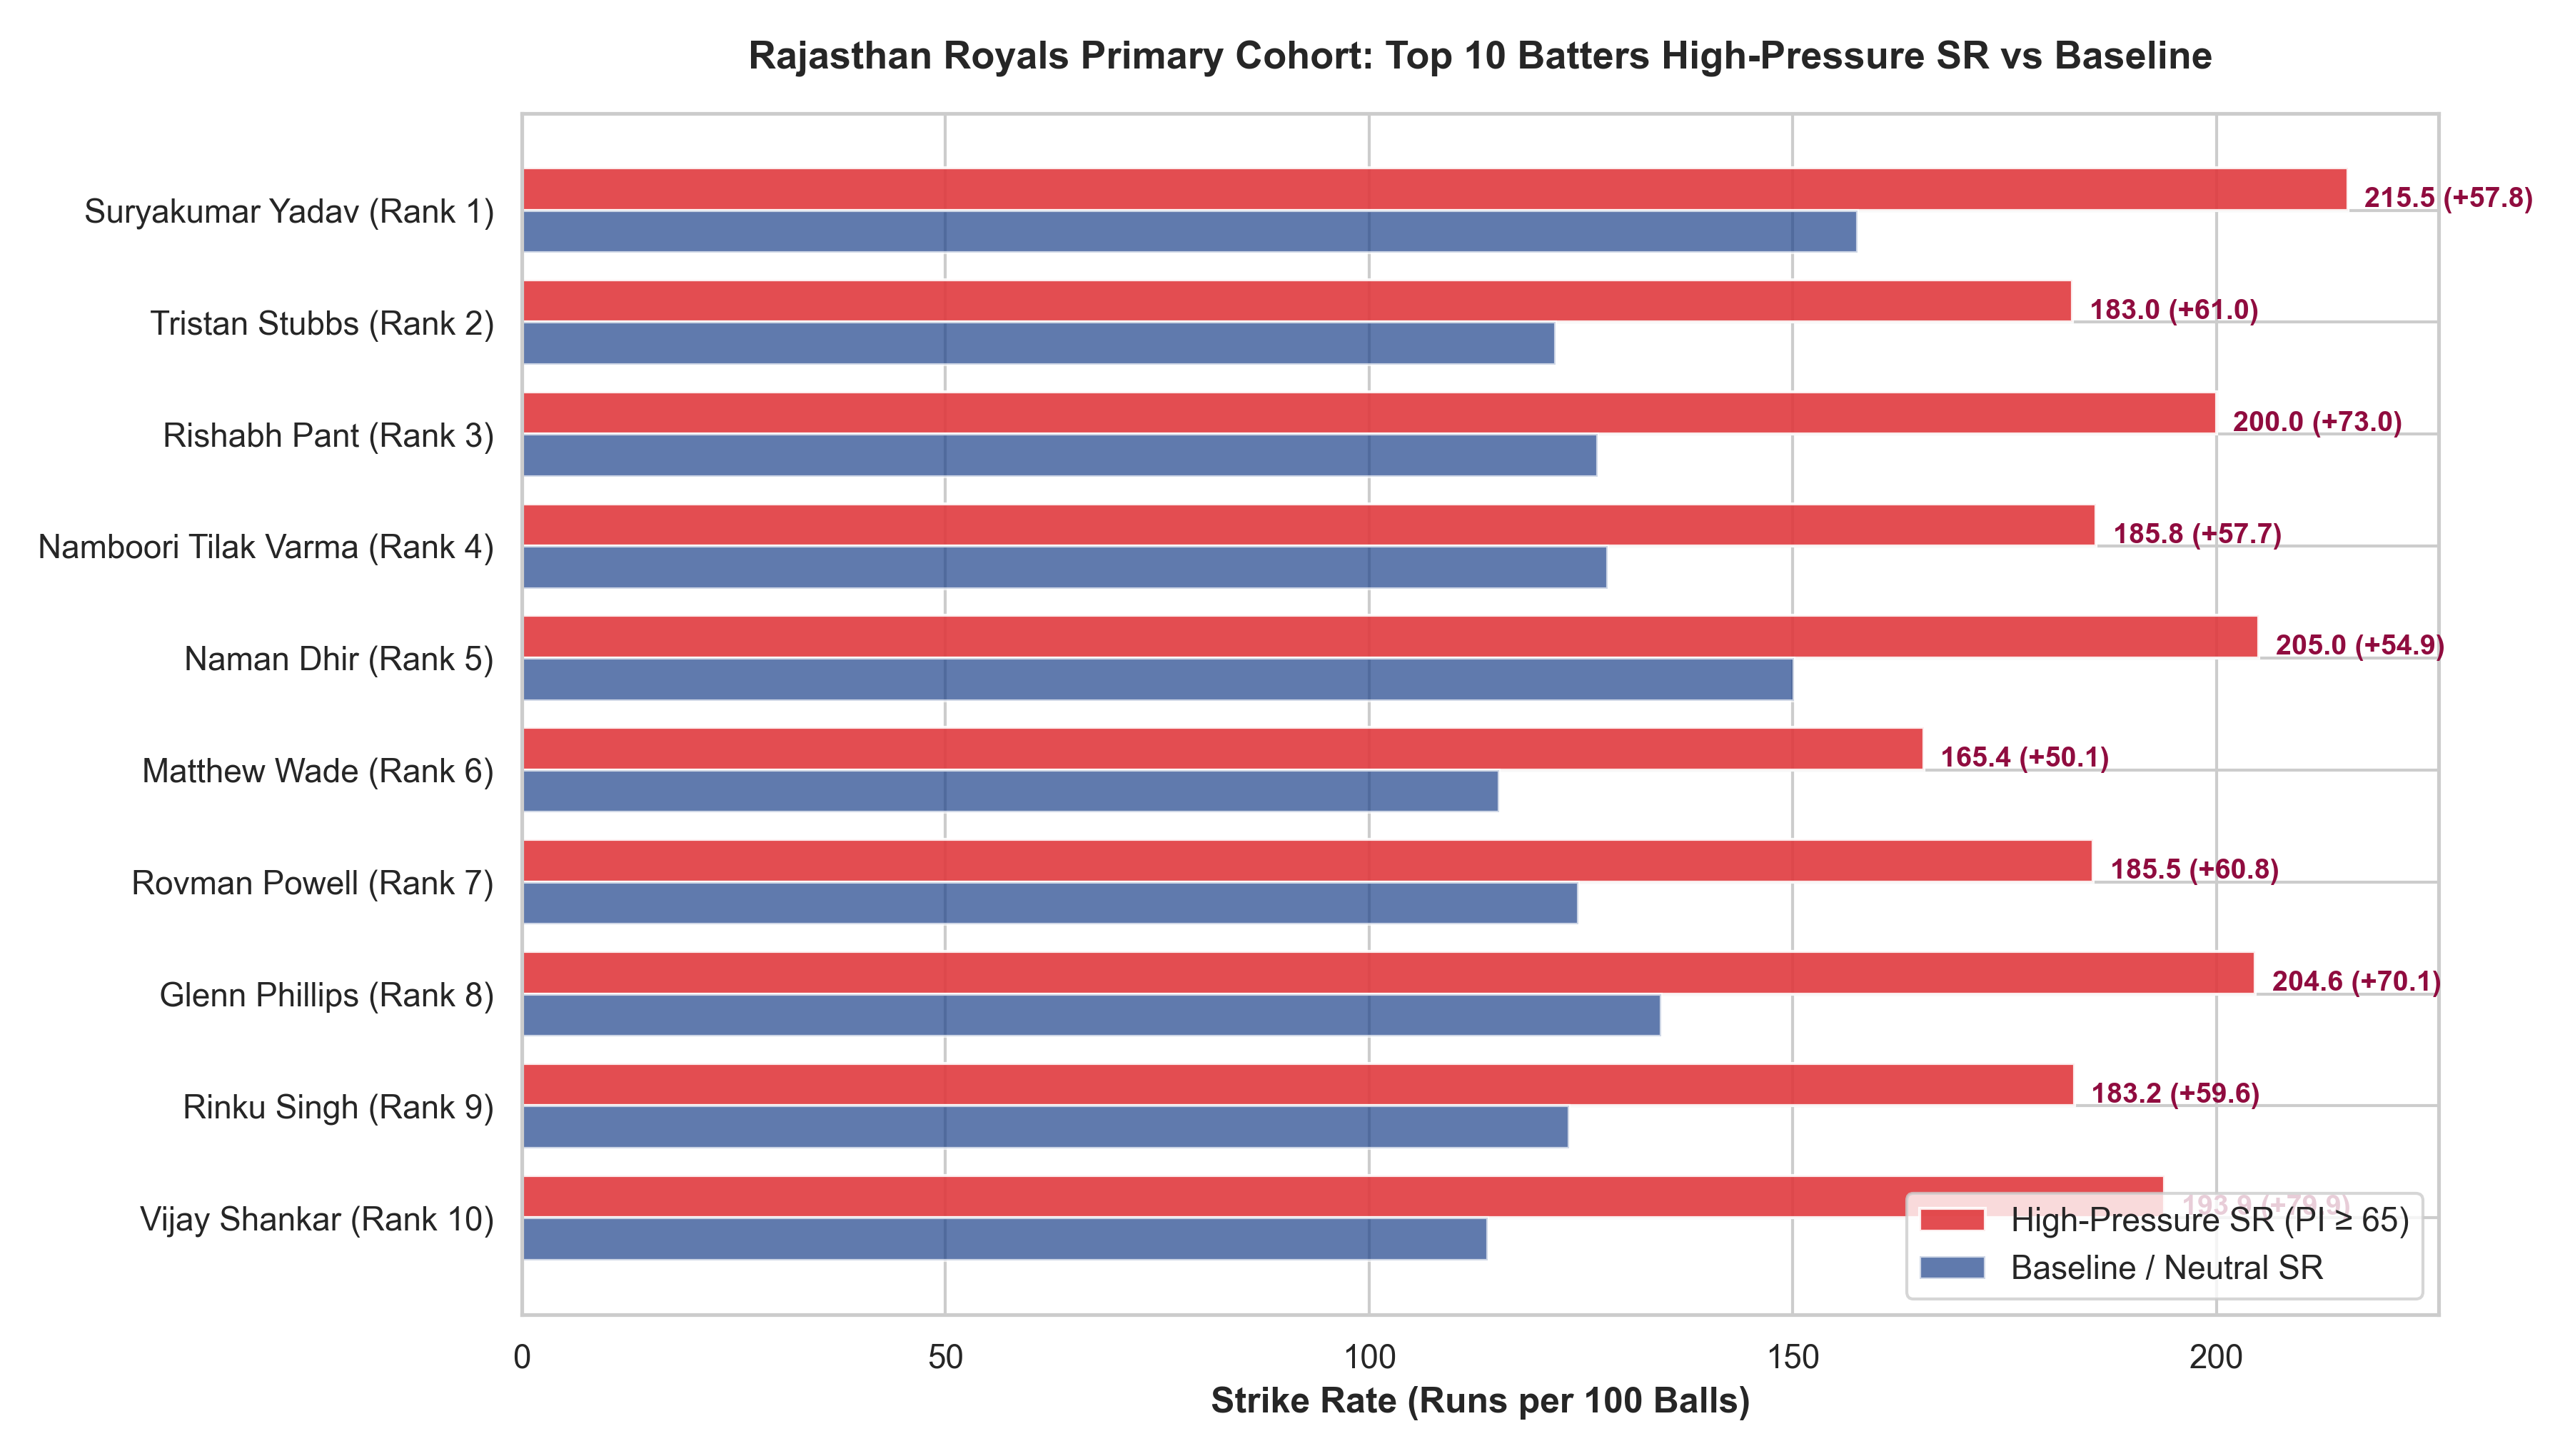
\includegraphics[width=\linewidth]{visualizations/top_10_batters_strike_rates.png}
        \caption{Batting Strike Rate under High Pressure vs Baseline ($\Delta SR$).}
        \label{fig:bat_sr}
    \end{subfigure}
    \hfill
    \begin{subfigure}[b]{0.48\textwidth}
        \centering
        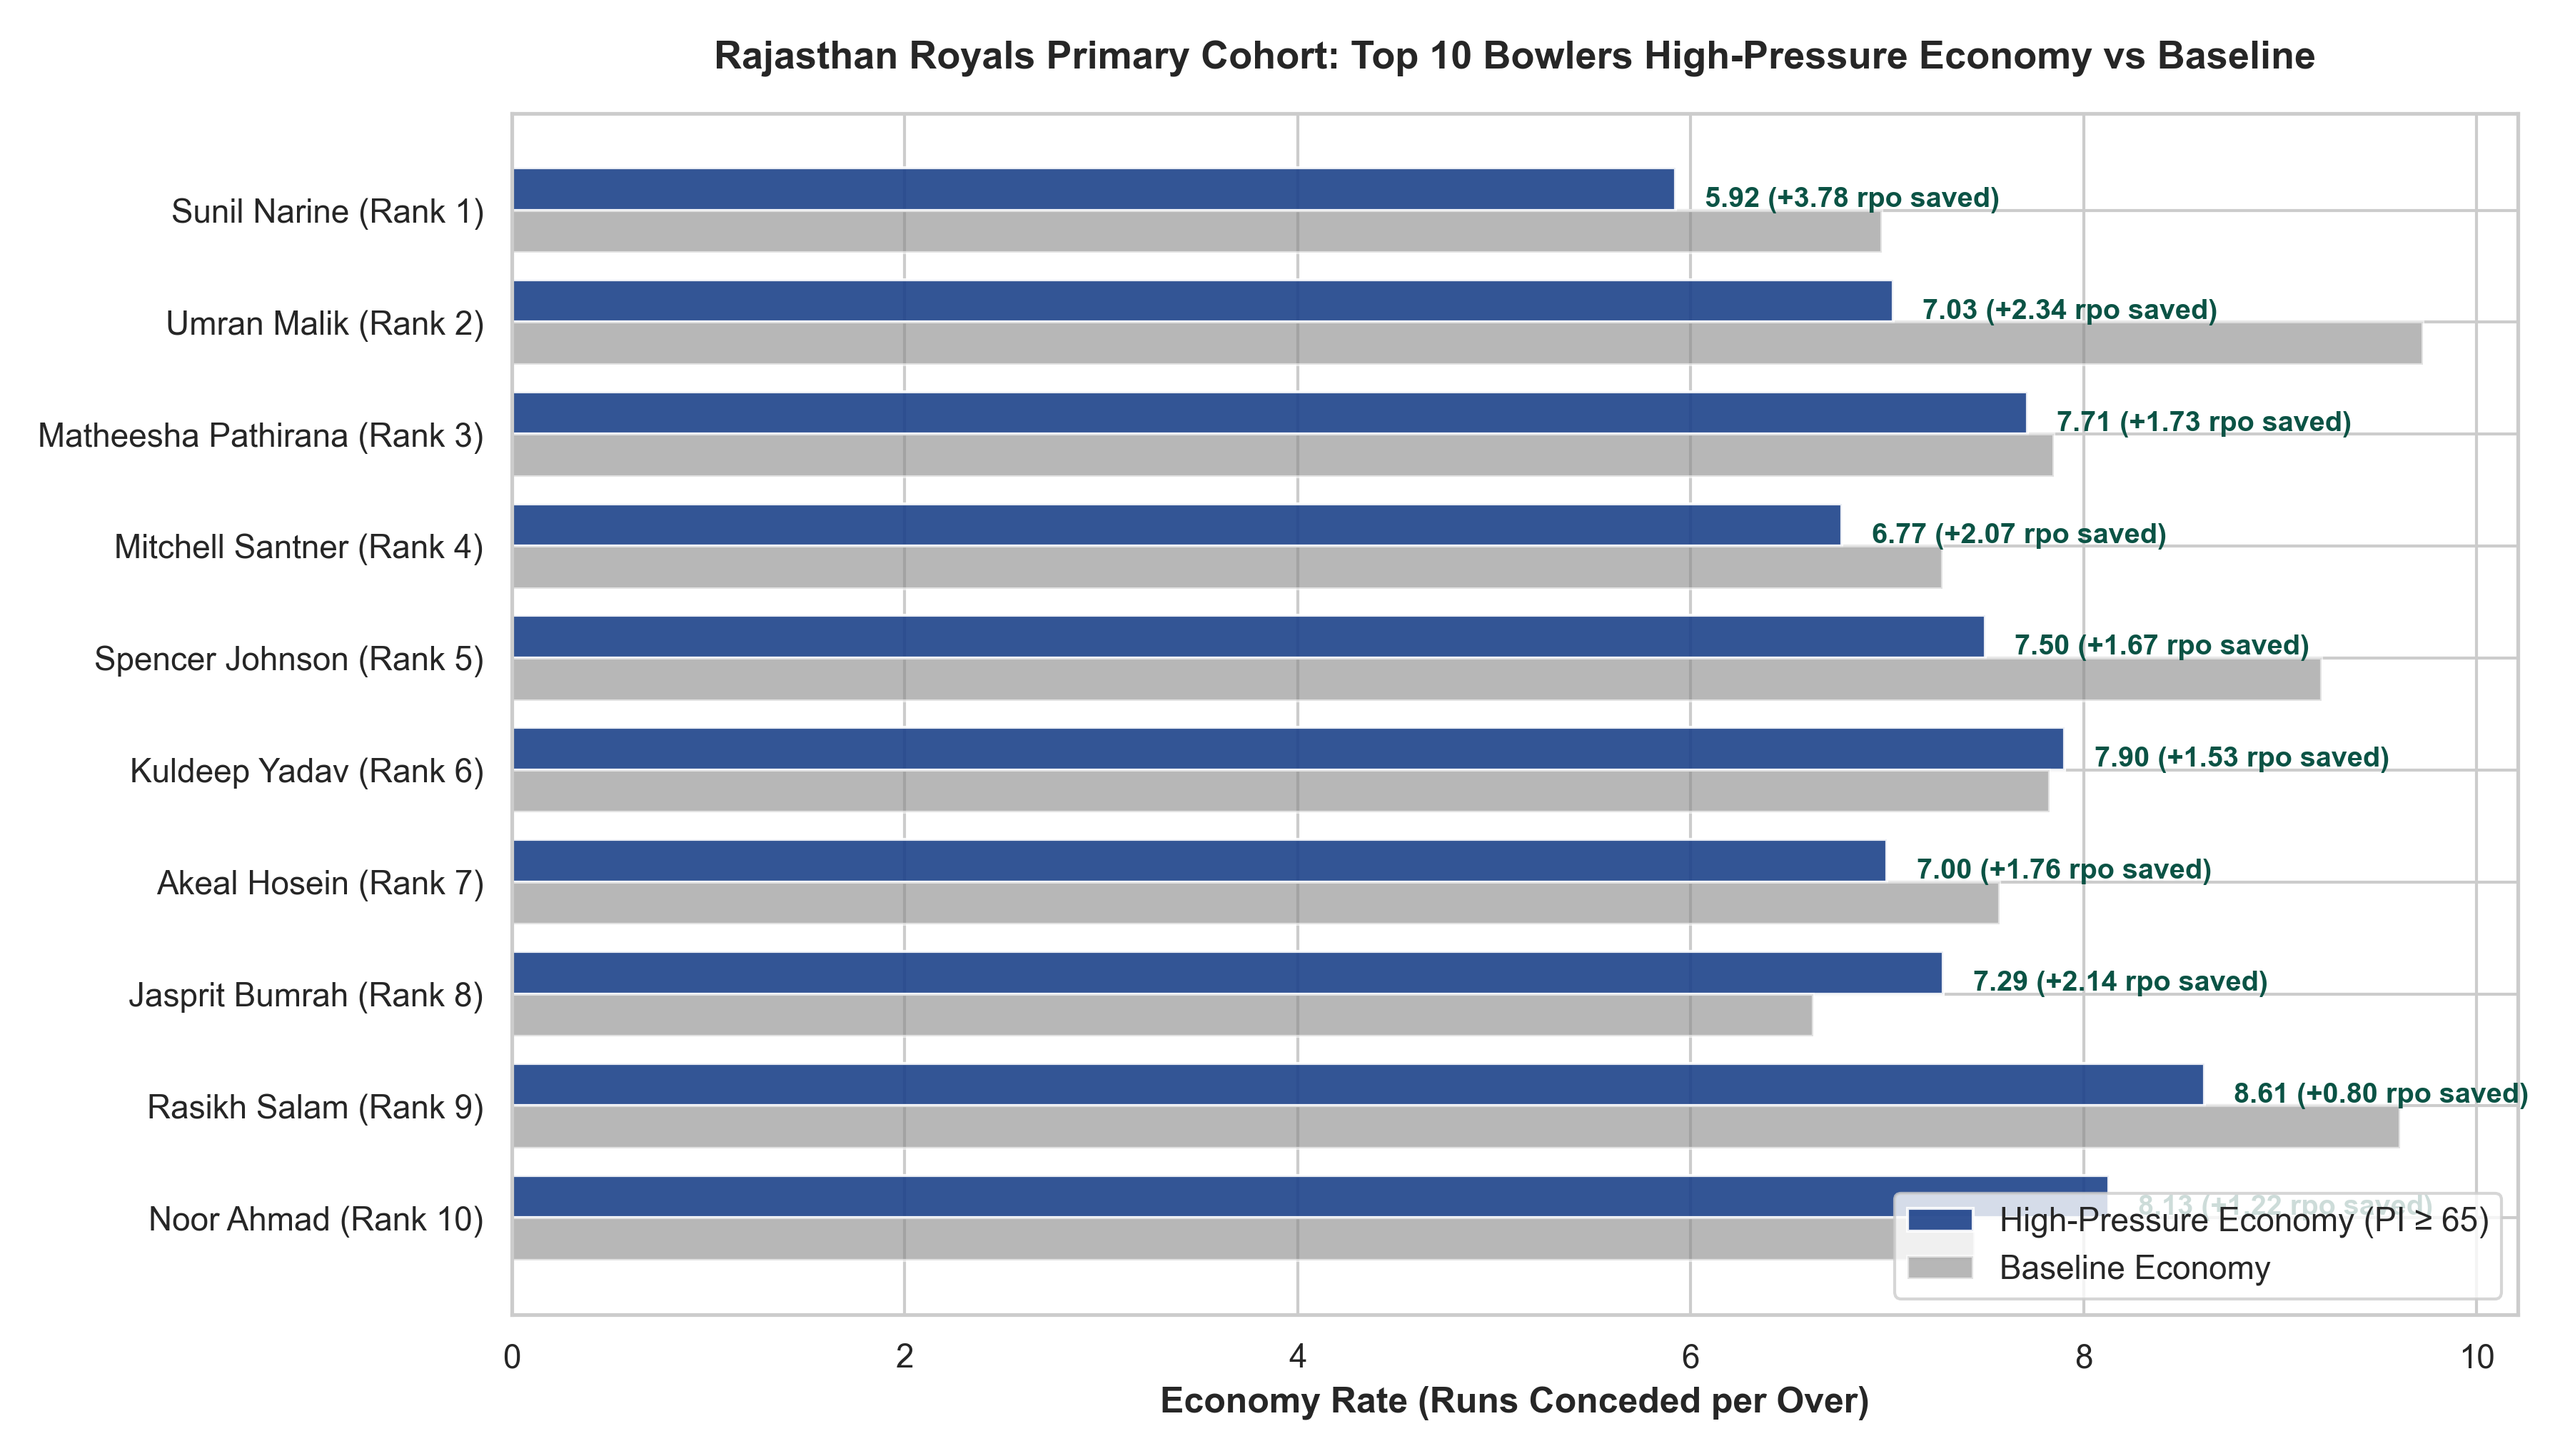
\includegraphics[width=\linewidth]{visualizations/top_10_bowlers_economy.png}
        \caption{Bowling Economy Rate under High Pressure vs Baseline ($\Delta Econ$).}
        \label{fig:bowl_econ}
    \end{subfigure}
    \caption{Clutch performance elevation profiles for top-ranked performers.}
    \label{fig:clutch_profiles}
\end{figure*}

\newpage

% ==============================================================================
% SECTION 6: TACTICAL DOSSIERS
% ==============================================================================
\section{Tactical Dossiers \& Forensic Player Profiles}

\subsection{Batting Highlights}
\paragraph{Suryakumar Yadav (IPL Rank 1 | Rating: 84.75)}
Across 426 high-pressure deliveries in the IPL and international cricket, SKY scores at an extraordinary strike rate of \textbf{215.49} ($+57.84$ delta above his $157.65$ baseline) with an average of $34.00$, hitting boundaries on \textbf{34.27\% of deliveries} (one boundary every 2.9 balls). In $74.4\%$ of high-pressure matches, his contributions were net-positive.

\paragraph{Tristan Stubbs (IPL Rank 2 | Rating: 73.24)}
Stubbs embodies death-overs batting efficiency. Facing 489 high-pressure deliveries, he maintains a \textbf{183.03 HP SR} ($+61.03$ delta) and $38.91$ average. His dot-ball rate is restricted to just \textbf{22.09\%}, demonstrating high strike rotation under pressure.

\paragraph{Rishabh Pant (IPL Rank 3 | Rating: 73.06)}
Pant exhibits a $+73.03$ strike rate delta under leverage, elevating his scoring from a $126.97$ baseline to \textbf{200.00 SR} across 274 pressure balls with an average of $32.24$ and $31.02\%$ boundaries.

\paragraph{Namboori Tilak Varma (IPL Rank 4 | Rating: 72.57)}
Tilak absorbed the highest pressure volume in the dataset: \textbf{634 balls and 1,178 runs} across 59 matches. Sustaining an \textbf{185.80 SR} ($+57.67$ delta) and $36.81$ average, he provides middle-order crisis stability.

\paragraph{Rovman Powell (IPL Rank 7 | Rating: 68.53)}
A core asset for Rajasthan Royals, Powell faced 572 high-pressure balls, amassing \textbf{1,061 runs at 185.49 SR} ($+60.77$ delta) with 84 sixes.

\subsection{Bowling Highlights}
\paragraph{Sunil Narine (IPL Rank 1 | Rating: 97.05)}
Narine delivers the most dominant pressure-containment profile in modern franchise cricket. Over 310 high-pressure balls, he concedes an economy of \textbf{5.92 rpo} (saving \textbf{$+3.78$ runs/over} relative to format expectations), taking 24 wickets at 12.92 balls per dismissal with \textbf{44.19\% dot balls}. In \textbf{90.7\%} of matches, his spells were net-positive.

\paragraph{Umran Malik (IPL Rank 2 | Rating: 86.59)}
Under high pressure, Malik's economy contracts to \textbf{7.03 rpo} ($+2.70$ improvement over his $9.73$ baseline) while his strike rate drops to \textbf{7.88 balls per wicket} (17 wickets in 134 balls, $52.24\%$ dots).

\paragraph{Matheesha Pathirana (IPL Rank 3 | Rating: 80.04)}
Pathirana is the premier death-overs pace weapon. Across 560 pressure balls, he captured \textbf{50 wickets} (11.20 strike rate) while maintaining a $7.71$ economy against elite death hitters ($80.5\%$ consistency rate).

\paragraph{Spencer Johnson (IPL Rank 5 | Rating: 73.95)}
Johnson registered a \textbf{7.50 HP economy} ($+1.67$ runs saved/over), a $10.67$ bowling strike rate, and a \textbf{92.3\% match win impact rate}.

% ==============================================================================
% SECTION 7: RELIABILITY, REPEATABILITY & LIMITATIONS
% ==============================================================================
\section{Reliability, Repeatability \& Model Limitations}

\subsection{Cross-Match Repeatability \& Opponent Breadth}
To guard against single-match outliers:
\begin{enumerate}[leftmargin=*,itemsep=2pt]
    \item \textbf{Positive Impact Match Rate:} Every player in our Top 10 maintained a positive context contribution across $50.0\%$ to $93.3\%$ of their high-pressure matches (averaging $74.2\%$ for batters and $84.8\%$ for bowlers).
    \item \textbf{Opposition Diversity:} All selected players executed under pressure across 8 to 17 unique international and franchise opponents.
    \item \textbf{Innings Balance:} Selected batters proved effective both setting targets and chasing. Tilak Varma faced 319 balls in Innings 1 and 315 in Innings 2; Suryakumar Yadav faced 240 balls in Innings 1 and 186 in Innings 2.
\end{enumerate}

\subsection{Model Limitations}
We acknowledge three inherent data constraints:
\begin{itemize}[leftmargin=*,itemsep=2pt]
    \item \textbf{Absence of Optical Trajectory Data:} The dataset lacks Hawk-Eye coordinates (pitch length, release height, lateral movement). Metrics measure outcome execution rather than pitch map mechanics.
    \item \textbf{Fielding Variance:} Unrecorded dropped catches and fielding misjudgments inject unmodeled variance into bowler economy and batter dismissals.
    \item \textbf{Sample Disparities:} Established stars carry narrower Bayesian credible intervals than emerging prospects, though our Empirical Bayes shrinkage ($K = 60$) regularizes this divergence.
\end{itemize}

% ==============================================================================
% SECTION 8: RAJASTHAN ROYALS ROSTER INTEGRATION & AUCTION STRATEGY
% ==============================================================================
\section{Franchise Roster Integration \& Auction Strategy}

Translating these findings into Rajasthan Royals' squad dynamics yields four clear operational directives:
\begin{enumerate}[leftmargin=*,itemsep=3pt]
    \item \textbf{Reconstructing Death Pace Firepower:} Wicket-taking suppresses death-overs scoring more effectively than defensive boundary containment. Matheesha Pathirana (50 pressure wickets, $11.20$ BSR) and Spencer Johnson ($7.50$ Econ, $92.3\%$ win rate) represent primary overseas pace targets to partner with Sandeep Sharma.
    \item \textbf{Middle-Overs Spin Choke Engine:} Spin containment remains the most reliable mechanism to stall high-pressure chases. Mitchell Santner ($6.77$ Econ, $+2.07$ runs saved/over) and Kuldeep Yadav (34 pressure wickets, $38.1\%$ dots) provide guaranteed run suppression.
    \item \textbf{Targeting Batters with Positive Clutch Deltas ($\Delta SR > +50$):} Unadjusted strike rates are misleading. Rajasthan Royals should prioritize hitters who accelerate under pressure. Tristan Stubbs ($+61.03$), Rishabh Pant ($+73.03$), and Naman Dhir ($+54.90$) exhibit statistically verified clutch elevation.
    \item \textbf{Strategic Validation of Rovman Powell:} Powell's ranking at \#7 among IPL batters with 572 high-pressure balls and a $+60.77$ strike rate delta quantitatively vindicates his vital tactical role in Rajasthan Royals' middle order.
\end{enumerate}

% ==============================================================================
% SECTION 9: CONCLUSION & VERIFICATION
% ==============================================================================
\section{Conclusion \& Submission Verification}
This investigation establishes a complete, mathematically grounded talent discovery framework for Round 1 of SupeRR Selector Season 2. Every player identifier has been cross-referenced with \texttt{competition\_team\_player\_mapping.csv} for seamless Unstop dropdown selection.

By combining dynamic win-probability leverage, gradient boosted expected values, empirical format calibration, and Bayesian shrinkage, Rajasthan Royals possesses a definitive analytical edge in discovering championship-winning clutch performers.

% ==============================================================================
% BIBLIOGRAPHY
% ==============================================================================
\begin{thebibliography}{99}
\bibitem{stern2016}
S.~E.~Stern, ``The Duckworth--Lewis--Stern method: An updated review,'' \emph{Journal of the Operational Research Society}, vol.~67, no.~11, pp.~1418--1428, 2016.
\bibitem{beaudoin2010}
D.~Beaudoin and T.~B.~Swartz, ``Strategies for cricket matches,'' \emph{The American Statistician}, vol.~64, no.~3, pp.~241--248, 2010.
\bibitem{davis2015}
J.~Davis, H.~Perera, and T.~B.~Swartz, ``A simulator for Twenty20 cricket,'' \emph{Australian \& New Zealand Journal of Statistics}, vol.~57, no.~1, pp.~55--69, 2015.
\bibitem{ke2017}
G.~Ke, Q.~Meng, T.~Finley, T.~Wang, W.~Chen, W.~Ma, Q.~Ye, and T.~Y.~Liu, ``LightGBM: A highly efficient gradient boosting decision tree,'' \emph{Advances in Neural Information Processing Systems}, vol.~30, pp.~3146--3154, 2017.
\bibitem{chen2016}
T.~Chen and C.~Guestrin, ``XGBoost: A scalable tree boosting system,'' in \emph{Proc. 22nd ACM SIGKDD Int. Conf. Knowl. Discovery Data Mining}, 2016, pp.~785--794.
\bibitem{prokhorenkova2018}
L.~Prokhorenkova, G.~Gusev, A.~Vorobev, A.~V.~Dorogush, and A.~Gulin, ``CatBoost: Unbiased boosting with categorical features,'' in \emph{Advances in Neural Information Processing Systems}, vol.~31, 2018, pp.~6638--6648.
\bibitem{gelman2013}
A.~Gelman, J.~B.~Carlin, H.~S.~Stern, D.~B.~Dunson, A.~Vehtari, and D.~B.~Rubin, \emph{Bayesian Data Analysis}, 3rd~ed., CRC Press, 2013.
\end{thebibliography}

\end{document}
